% no answer key
\documentclass[letterpaper]{exam}

% answer key
% \documentclass[letterpaper, landscape]{exam}
% \usepackage{2in1, lscape} 
% \printanswers

\usepackage{units} 
\usepackage{xfrac} 
\usepackage[fleqn]{amsmath}
\usepackage{float}
\usepackage{mdwlist}
\usepackage{booktabs}
\usepackage{cancel}
\usepackage{polynom}
\usepackage{caption}
\usepackage{fullpage}
\usepackage{comment}
\usepackage{enumerate}
\usepackage{graphicx}
\usepackage{mathtools} 

\addpoints

\newcommand{\dg}{\ensuremath{^\circ}} 
\newcommand{\sgn}{\operatorname{sgn}}

\everymath{\displaystyle}
\title{Calculus I \\ Exam One}
\author{}
\date{\today}

\begin{document}

  \maketitle

  % \begin{center}
  %   \gradetable[h][pages]
  % \end{center}

  \begin{questions}

    \question 
    \label{q:limits}

      \begin{figure}[H]
        \centering
        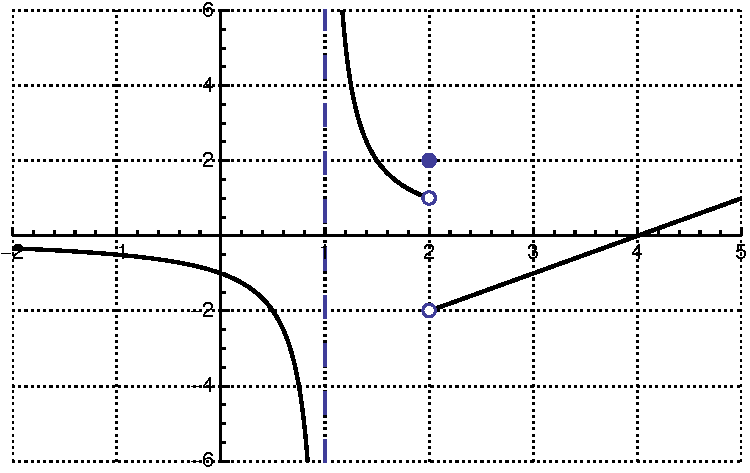
\includegraphics[scale = 0.6]{limits.pdf}
        \caption{Question~\ref{q:limits}}
        \label{fig:limits}
      \end{figure}
      
      See Figure~\ref{fig:limits}. Find each limit or explain why it does not exist. 

      \begin{parts}
        \part[2] $\lim_{x \to 1^{-}} f(x)$
          \begin{solution}
            $lim_{x \to 1^-} f(x) = -\infty$
          \end{solution}

        \part[2] $\lim_{x \to 1^{+}} f(x)$
          \begin{solution}
            $lim_{x \to 1^+} f(x) = \infty$
          \end{solution}

        % \part[2] $\lim_{x \to 1} f(x)$
        %   \begin{solution}
        %     $lim_{x \to 1} f(x)$ is not defined since the right hand and left hand limits are different.
        %   \end{solution}
          
        \part[2] $\lim_{x \to 2^{-}} f(x)$
          \begin{solution}
            $lim_{x \to 2^-} f(x) = 1$
          \end{solution}

        \part[2] $\lim_{x \to 2^{+}} f(x)$
          \begin{solution}
            $lim_{x \to 2^+} f(x) = -2$
          \end{solution}

        \part[2] $\lim_{x \to 2} f(x)$
          \begin{solution}
            $lim_{x \to 2} f(x)$ is not defined since the right hand and left hand limits are different.
          \end{solution}
          
      \end{parts}

    \uplevel{For questions \ref{q:first_limit} to \ref{q:last_limit} find each limit.}

    \question[7] 
    \label{q:first_limit}
      \[
        \lim_{x \to 2} \frac{x^2 + x - 6}{x^2 - 5x + 6}
      \]

      \begin{solution}
        \begin{align*}
          \lim_{x \to 2} \frac{x^2 + x - 6}{x^2 - 5x + 6}  & = \lim_{x \to 2} \frac{(x + 3)(x - 2)}{(x - 2)(x - 3)} \\
                                                           & = \lim_{x \to 2} \frac{x + 3}{x - 3} \\
                                                           & = \boxed{ -5 } \\
        \end{align*}
      \end{solution}

    \question[10]
      \[
        \lim_{x \to 2} \frac{x^4 - 16}{x^2 - 3x + 2}
      \]

      \begin{solution}
        \begin{align*}
          \lim_{x \to 2} \frac{x^4 - 16}{x^2 - 3x + 2} & = \lim_{x \to 2} \frac{\left( x^2 - 4\right) \left( x^2 + 4 \right)}{(x - 2)(x - 1)} \\
                                                       & = \lim_{x \to 2} \frac{(x + 2) (x - 2) \left( x^2 + 4 \right)}{(x - 2)(x - 1)} \\
                                                       & = \lim_{x \to 2} \frac{(x + 2) \left( x^2 + 4 \right)}{x - 1} \\
                                                       & = \boxed{ 32 } \\
        \end{align*}
      \end{solution}

    \question[10]
      \[
        \lim_{x \to 0} \frac{1}{x^2 - 2x} + \frac{1}{2x}
      \]

      \begin{solution}
        \begin{align*}
        \lim_{x \to 0} \frac{1}{x^2 - 2x} + \frac{1}{2x} & = \lim_{x \to 0} \frac{2x + x^2 - 2x}{2x\left( x^2 - 2x \right)} \\
                                                         & = \lim_{x \to 0} \frac{x^2}{2x \left( x^2 - 2x \right)} \\
                                                         & = \lim_{x \to 0} \frac{x^2}{2x^2 (x - 2)} \\
                                                         & = \lim_{x \to 0} \frac{1}{2x - 4} \\
                                                         & = \boxed{ - \frac{1}{4} } \\
        \end{align*}
      \end{solution}


    \question[7]
      \[
        \lim_{x \to 1^-} \frac{|x - 1|}{x - 1}
      \]

      \begin{solution}
        Notice that when $x$ is less than 1, $x - 1$ is negative and $|x - 1| = - (x - 1)$.

        \begin{align*}
          \lim_{x \to 1^-} \frac{|x - 1|}{x - 1} & = \lim_{x \to 1^-} \frac{- (x - 1)}{x - 1} \\
                                                 & = - \lim_{x \to 1^-} \frac{x - 1}{x - 1} \\
                                                 & = \boxed{ -1 } \\
        \end{align*}
      \end{solution}

    % \question[7] 
    %   \[
    %     \lim_{x \to 9} \frac{9 - x}{\sqrt{x} - 3} 
    %   \]

    %   \begin{solution}
    %     \begin{align*}
    %       \lim_{x \to 9} \frac{9 - x}{\sqrt{x} - 3}  & = \lim_{x \to 9} \frac{\left( 3 + \sqrt{x} \right) \left( 3 - \sqrt{x} \right)}{\sqrt{x} - 3} \\
    %                                                  & = - \lim_{x \to 9} \frac{\left( 3 + \sqrt{x} \right) \left( \sqrt{x} - 3 \right)}{\sqrt{x} - 3} \\
    %                                                  & = - \lim_{x \to 9} \left( 3 + \sqrt{x} \right) \\
    %                                                  & = \boxed{ -6 }
    %     \end{align*}
    %   \end{solution}

    \question[7] 
    \label{q:last_limit}
      \[
        \lim_{x \to \infty} \frac{2x^3 + 3x - 7}{2x^2 - 3x^3}
      \]

      \begin{solution}
        \begin{align*}
          \lim_{x \to \infty} \frac{2x^3 + 3x - 7}{2x^2 - 3x^3} & = \lim_{x \to \infty} \frac{2 + 3/x^2 - 7/x^3}{2/x - 3} \\
                                                                & = \boxed{ - \frac{2}{3} } \\
        \end{align*}
      \end{solution}

    \question[5] Does $x^2 - \sqrt{x + 1} = 0$ have a solution between $x = -1$ and $x = 1$?

    \question[10]
      Prove, using the precise definition of a limit ($\epsilon$/$\delta$ proof) that:
      \[
        \lim_{x \to 1} 2x + 1 = 3
      \]

      \begin{solution}
        Show that for all $\epsilon$ there is a $\delta$ such that if 
        $0 < |x - 1| < \delta$ 
        
        then $|(2x + 1) - 3| < \epsilon$

        \paragraph{preliminary investigation}
        \begin{align*}
          |(2x + 1) - 3| & = 2|x - 1| \\
          \delta         & = \frac{\epsilon}{2} \\
        \end{align*}

        \paragraph{proof}
        Show that if $\delta = \frac{\epsilon}{2}$ and $0 < |x - 1| < \delta$

        then $|(2x + 1) - 3| < \epsilon$
        \[
          |(2x + 1) - 3| = 2|x - 1| < 2 \delta = 2 \cdot \frac{\epsilon}{2} = \epsilon
        \]
        
      \end{solution}

    \question[8]
    \label{q:continuity}
      \[
          f(x) =
            \begin{cases}
              x - 1,        & \text{ if } x \leq 1 \\
              x^2 - 1,      & \text{ if } 1 < x < 3 \\
              \sqrt{x - 3}, & \text{ if } x \geq 3 \\
            \end{cases}
      \]

      Find the numbers where $f$ is discontinuous. At which of these numbers is $f$
      continuous from the right, left, or neither?

      \begin{solution}
        \begin{figure}[H]
          \centering
          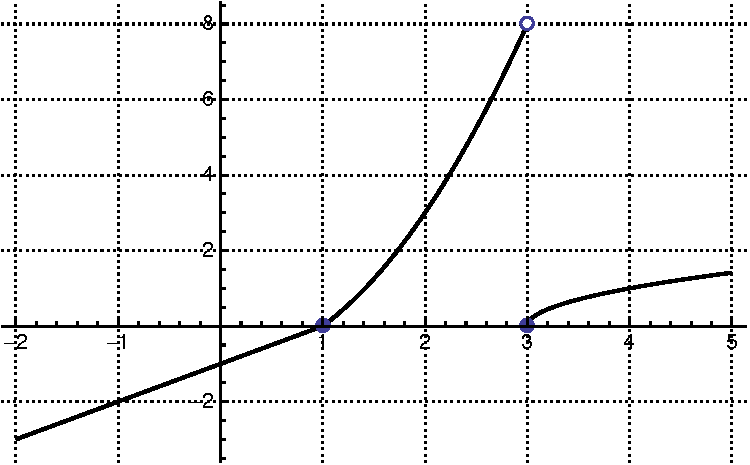
\includegraphics[scale = 0.5]{continuity.pdf}
          \caption{Question~\ref{q:continuity}}
          \label{fig:continuity}
        \end{figure}

        $f$ is discontinuous at $x = 3$. At this point $x$ is continuous from the right
        but not from the left.

      \end{solution}

      \uplevel{For questions \ref{derivative:first} to \ref{derivative:last}, use the
      definition of the derivative to find $f'(x)$}

      \question[8] 
      \label{derivative:first}
      \[
        f(x) = x^2 + 2x - 5
      \]

      \begin{solution}
        \begin{align*}
          f'(x) & = \lim_{h \to 0} \frac{(x + h)^2 + 3(x + h) - 5 - \left( x^2 + 3x - 5 \right)}{h} \\
                & = \lim_{h \to 0} \frac{x^2 + 2xh + h^2 + 3(x + h) - 5 - \left( x^2 + 3x - 5 \right)}{h} \\
                & = \lim_{h \to 0} \frac{2xh + h^2 + 3h}{h} \\
                & = \lim_{h \to 0} (2xh + 3 + h) \\
                & = \boxed{ 2x + 3 } \\
        \end{align*}
      \end{solution}

      \question[8] 
      \label{derivative:last}
      \[
        f(x) = 1 - \frac{2}{x}
      \]

      \begin{solution}
        \begin{align*}
          f'(x) & = \lim_{h \to 0} \frac{1 - \frac{2}{x + h} - \left( 1 - \frac{2}{x} \right)}{h} \\
                &= \lim_{h \to 0} \frac{\frac{2}{x} - \frac{2}{x+h}}{h} \\
                &= \lim_{h \to 0} \frac{2x + 2h - 2x}{hx(x + h)} \\
                &= \lim_{h \to 0} \frac{2}{x(x + h)} \\
                &= \boxed{ \frac{2}{x^2} } \\
        \end{align*}
      \end{solution}
      
      \question[10] Find an equation of the tangent to $y = \sqrt{x}$ at the point $(1, 1)$
      \begin{solution}
        \begin{align*}
          f'(x) & = \lim_{h \to 0} \frac{\sqrt{x + h} - \sqrt{x}}{h} \\
                & = \lim_{h \to 0} \frac{\sqrt{x + h} - \sqrt{x}}{h} \cdot \frac{\sqrt{x + h} + \sqrt{x}}{\sqrt{x + h} + \sqrt{x}} \\
                & = \lim_{h \to 0} \frac{x + h - x}{h \left( \sqrt{x + h} + \sqrt{x} \right)} \\
                % & = \lim_{h \to 0} \frac{h}{h \left( \sqrt{x + h} + \sqrt{x} \right)} \\
                & = \lim_{h \to 0} \frac{1}{ \sqrt{x + h} + \sqrt{x} } \\
                & = \frac{1}{2 \sqrt{x}} \\
          \\
          f'(1) &= \frac{1}{2} \\
          \\
          \frac{1}{2} & = \frac{y - 1}{x - 1} \\
          y           & = \boxed{ \frac{x}{2} + \frac{1}{2} } \\
        \end{align*}
      \end{solution}

  \end{questions}

\end{document}

